\section{Introduction}
\label{s_motive}

In the 70 years since nuclear bombs were dropped on Hiroshima and Nagasaki, the knowledge and technology required to make these weapons has proliferated around the globe. There are now nine states that have developed their own nuclear weapons, as well as many others who have the capability to do so\cite{feiveson_unmaking_2014}.  Moreover, this knowledge will continue to spread as climate change change further tilts the scales such that the benefits of nuclear power outweigh the risks \cite{mooney_why_2014}.  China is already investing heavily in nuclear power, planning to triple its generating capacity from 19GWe to 58GWe by 2020  \cite{_china_2014}.  As climate change increasingly dominates discussions of national security, the perception of the risks inherent to nuclear energy is decreasing and states are embracing nuclear energy as a reliable large-scale source of carbon-neutral energy.  However, the expansion of nuclear power increases concerns with respect to nuclear security, because the same technologies used to produce nuclear fuel can also be exploited in the pursuit of nuclear weapons.


\subsection{Sensitive Parts of the Nuclear Fuel Cycle}

Two nuclear technologies are of of particular concern for proliferation, uranium enrichment and plutonium reprocessing.  Uranium enrichment is required for the once-through fuel cycles that are dominant around the world today, and used exclusively in the US.  A once-through fuel cycle includes a source of natural uranium such as a mine, and is comprised of non-fissile 99.3\% $^{238}U$ and only 0.7\% fissile $^{235}U$. Concentrations of 4-20\% fissile $^{235}U$ are required to fuel a nuclear reactor. Enrichment facilities are used to increase the concentration of $^{235}U$ to the desired amount.  Fuel is then burned in a nuclear reactor and the remaining material, which includes the original $^{238}U$, short- and long-lived fission products, as well as \~1\% $^{239}Pu$ and $^{240}Pu$, is then stored as waste.  The enrichment facility is notable because it can be used to increase the concentration of $^{235}U$ up to the 80-90\% required to make a nuclear weapon\cite{_military_2014}.

Several countries are developing nuclear reactors that can accomodate recycled fuel \cite{_processing_2015}.  Recycled fuel is plutonium-based rather than uranium-based, and is made by separating the components of spent uranium fuel and increasing the concentration of fissile $^{239}Pu$ up to 80\%.  This material can then be used as fuel or blended with uranium to make \gls{MOX}.  As with the enrichment process however, separations facilities can increase the concentration beyone that required for fuel to generate \gls{WGP} (up to 93\% $^{239}Pu$).  However, fuel cycles with the capability to burn \gls{MOX} fuel are advangteous because \gls{WGP} from decommissioned nuclear weapons can be blended into \gls{MOX}, which reduces the amount of \gls{SNM} that must be safeguarded.  In part due to the large stockpile of \gls{WGP} in the \gls{US}, reprocessessing has been considered at several times over the past half-century.  However, a host of political, economic, environmental and strategic concerns have cpushed the issue of reprocessing out of the technical realm and it has become a contentious political topic, and currently the \gls{US} is pursuing only basic science research in this field \cite{rossin_policy_????, editorial_adieu_2009}.
 
\subsection{Use of Treaties to Minimize Proliferation}

While it has not proven possible to prevent the spread of nuclear knowledge entirely, international treaties have been used in an attempt to control it.  The \gls{NPT}, which has been signed by 190 states including the original 5 nuclear weapons states, has codified a set of rules and norms for allowing the peaceful pursuit of nuclear energy\cite{_treaty_????}.  The \gls{NPT} created an organization called \gls{IAEA}, whose role is to verify compliance with the treaty by periodically inspecting facilities related to nuclear technology.  Other notable treaties include \gls{CTBT}, which placed a moratorium on testing nuclear weapons, and the \gls{START} in which the \gls{US} and Russia agreed on nuclear arms reductions.

These treaties seek to have done much to prevent the spread of nuclear weapons, but they do not address the production capabilities of states that already posess nuclear weapons.  A potential \gls{FMCT} would place limits on the amount of \gls{SNM} each weapons state could stockpile, possibly including current stockpiles in addition to future production.  However, a major unresolved issue is the difficulty of developing verification techniques that can reliably confirm that nuclear material is not being produced \cite{_fissile_2013}.  Furthermore, making measurements of nuclear material for treaty verification is itself a sensitive issue, as even collecting the spectra of a material to confirm its authenticity can potentially expose sensitive information\cite{glaser_zero-knowledge_2014}. Particularly if non-weapons states are to contribute to treaty verification, it is important to prevent the further dissemination of nuclear knowledge.

\begin{figure}%[htbp!]
\begin{center}
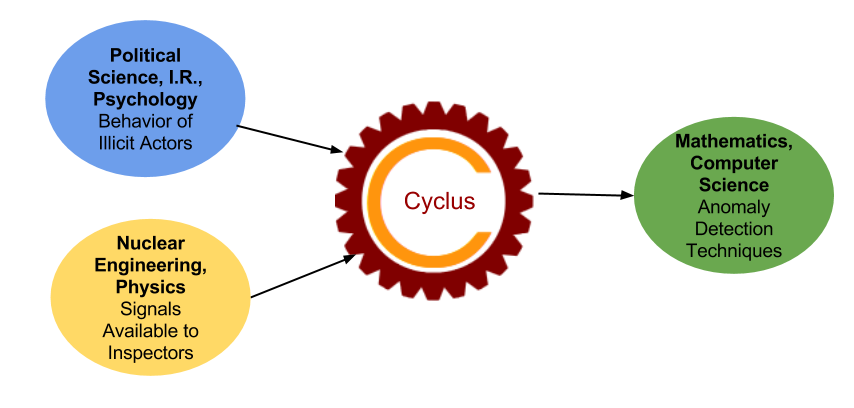
\includegraphics[natwidth=162bp,natheight=227bp, scale=0.5]{./figs/cyclus_interdiscipline.png}
\end{center}
\caption{The \Cyclus nuclear fuel cycle simulator provides a testbed to integrate innovations in treaty verification across many disciplines.}
\label{fig:cyclus_diagram}
\end{figure}

An effective treaty verification regime must synthesize knowledge from the realmns of political science, international relations, nuclear physics and engineering, and even behavioral psychology.  A nuclear fuel cycle simulator provides a framework in which to integrate these disparate components into an effective strategy.  As shown in Figure \ref{fig:cyclus_diagram}, a fuel cycle simulator can combine the technical specifications of innovative detection modalities, signal processing techniques, and models of the social-behavioral interactions between actors to provide insights into proposed verification approaches.  At a systems level, a fuel cycle simulator can be used to frame test scenarios as responses to stimuli. That is, even if not all of the specific details are available, simulations can incorporate response behaviors to illucidate the strengths and weaknesses of various verification strategies.


